\section{Constructive 4SID algorithm}

4SID for noise-free data was initially discovered in the 1960s; however, its applicability was limited due to its inability to handle noisy data effectively. 
It was later rediscovered in the 1990s with the advent of Singular Value Decomposition, a pivotal tool in numerical algebra.

Considering the practical scenario, let's address the real-world problem where impulse response experiments are affected by noise.
\begin{figure}[H]
    \centering
    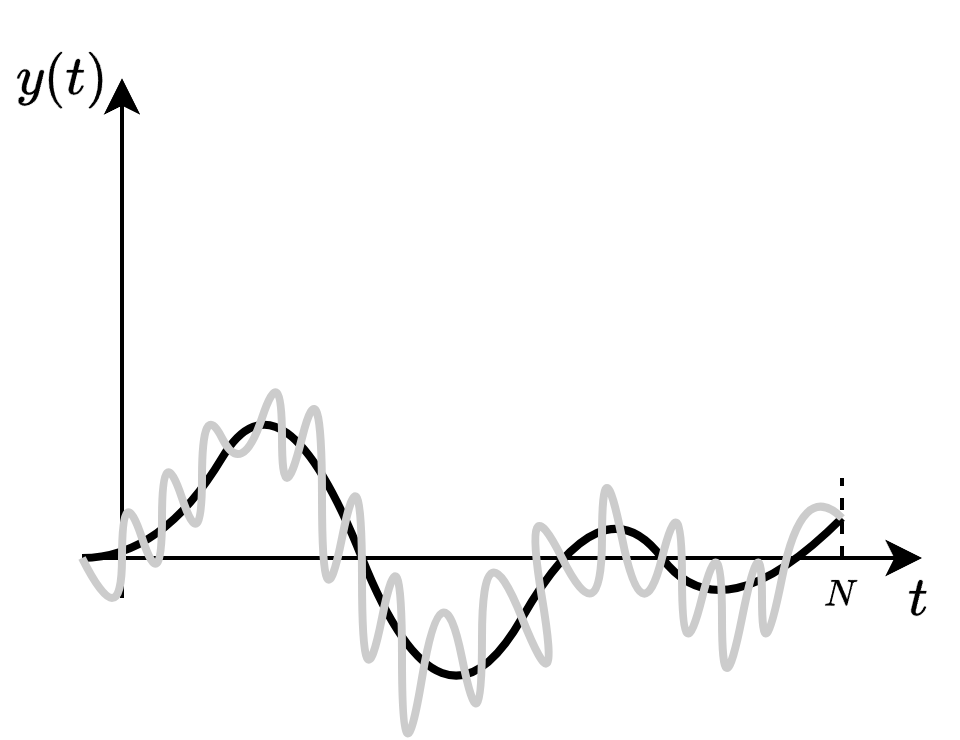
\includegraphics[width=0.5\linewidth]{images/noiserep.png}
    \caption{Real and ideal impulse response to a step input}
\end{figure}
In this context, each recorded impulse response data point consists of the true value along with a noise component:
\[\tilde{\omega}(t)=\omega(t)+\eta(t)\qquad t=0,1,2,\dots,N\]
Thus, the dataset is structured as follows:
\[\left\{ \tilde{\omega}(0),\tilde{\omega}(1),\tilde{\omega}(2),\dots,\tilde{\omega}(N)\right\}\]
Here, $N$ represents a minimum of 100 samples. 

\subsection{Algorithm}
Here's how the algorithm functions:
\begin{enumerate}
    \item Construct the Hankel matrix $\tilde{\mathbf{H}}_{qd}$ using the full dataset, we arrange the data in the following manner:
        \[\tilde{\mathbf{H}}_{qd}=\begin{bmatrix}
            \tilde{\omega}(1) & \tilde{\omega}(2) & \tilde{\omega}(3) & \cdots & \tilde{\omega}(d) \\ 
            \tilde{\omega}(2) & \tilde{\omega}(3) & \tilde{\omega}(4) & \cdots & \tilde{\omega}(d+1) \\ 
            \tilde{\omega}(3) & \tilde{\omega}(4) & \tilde{\omega}(5) & \cdots & \tilde{\omega}(d+2) \\ 
            \vdots & \vdots  & \vdots  & \vdots  & \vdots  \\ 
            \tilde{\omega}(q) & \tilde{\omega}(q+1) & \tilde{\omega}(q+2) & \cdots & \tilde{\omega}(q+d-1) \\ 
        \end{bmatrix}\]
        This matrix is diagonal with dimensions $q \times d$, where it's assumed that $q<d$. 
        Given the relation $q+d-1=N$, it follows that $q=N+1-d$.
        That graphically becomes: 
        \begin{figure}[H]
            \centering
            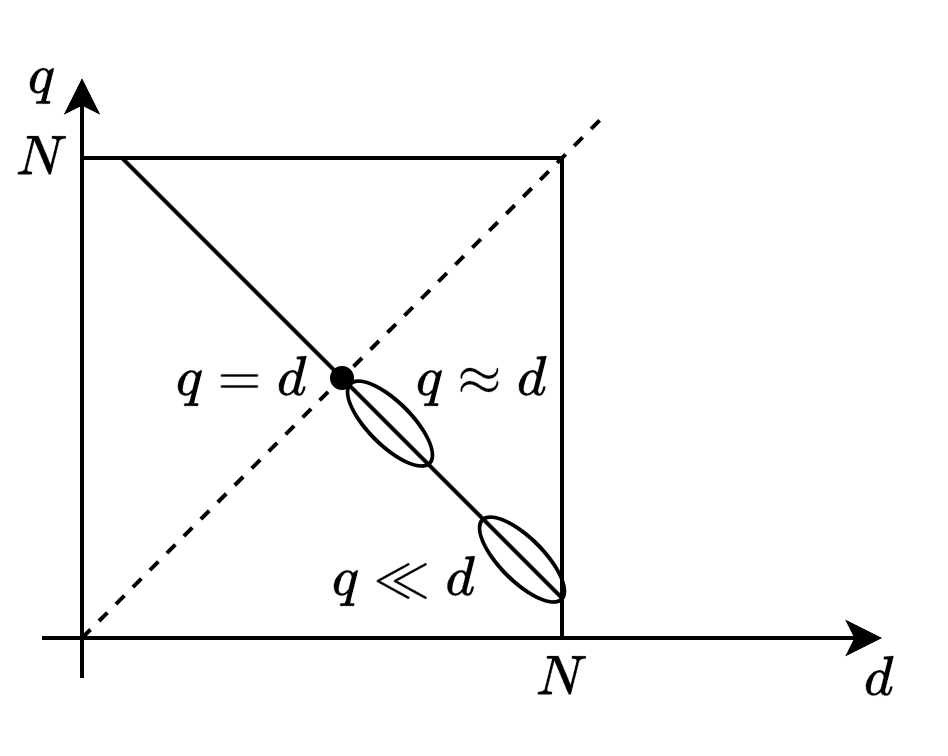
\includegraphics[width=0.4\linewidth]{images/qd.png}
            \caption{Graphical representation of the matrix dimension}
        \end{figure}
        When $q \ll d$, estimation quality is compromised but computational efficiency is maximized.
        When $q \approx d$, estimation quality is optimized but computational complexity increases.
        The optimal choice lies where $q>\frac{1}{2}d$, balancing estimation quality and computational efficiency.
        It's worth noting that there's only a minor sensitivity to the specific values of $q$ and $d$ as long as they adhere to this inequality.
    \item Singular Value Decomposition of the matrix $\tilde{\mathbf{H}}_{qd}$ is given by:
        \[\tilde{\mathbf{H}}_{qd}=\tilde{\mathbf{U}}\tilde{\mathbf{S}}\tilde{\mathbf{V}}^T\]
        Here, $\tilde{\mathbf{H}}_{qd}$ is a $q \times d$ matrix, $\tilde{\mathbf{U}}$ is a $q \times q$ unitary matrix, $\tilde{\mathbf{S}}$ is a $q \times d$ matrix, and $\tilde{\mathbf{V}}$ is a $d \times d$ unitary matrix. 
        The matrix $\tilde{\mathbf{S}}$ is defined as: 
        \[\tilde{\mathbf{S}}=\begin{bmatrix}
            \sigma_1 & 0 & 0 & \cdots & 0 & \cdots & 0\\ 
            0 & \sigma_2 & 0 & \cdots & 0 & \cdots & 0\\ 
            0 & 0 & \sigma_3 & \cdots & 0 & \cdots & 0\\ 
            \vdots & \vdots  & \vdots  & \ddots  & \vdots  & \vdots & \vdots\\ 
            0 & 0 & 0 & \cdots & \sigma_q & \cdots & 0\\ 
        \end{bmatrix}\]
        Here, $\sigma_1,\sigma_2,\cdots,\sigma_q$ are the singular values of matrix $\tilde{\mathbf{H}}_{qd}$, which are real positive numbers sorted in decreasing order: $\sigma_1\geq\sigma_2\geq\cdots\geq\sigma_q$. 
    \item Plot the singular values and identify the system part of the matrix. 
        \begin{figure}[H]
            \centering
            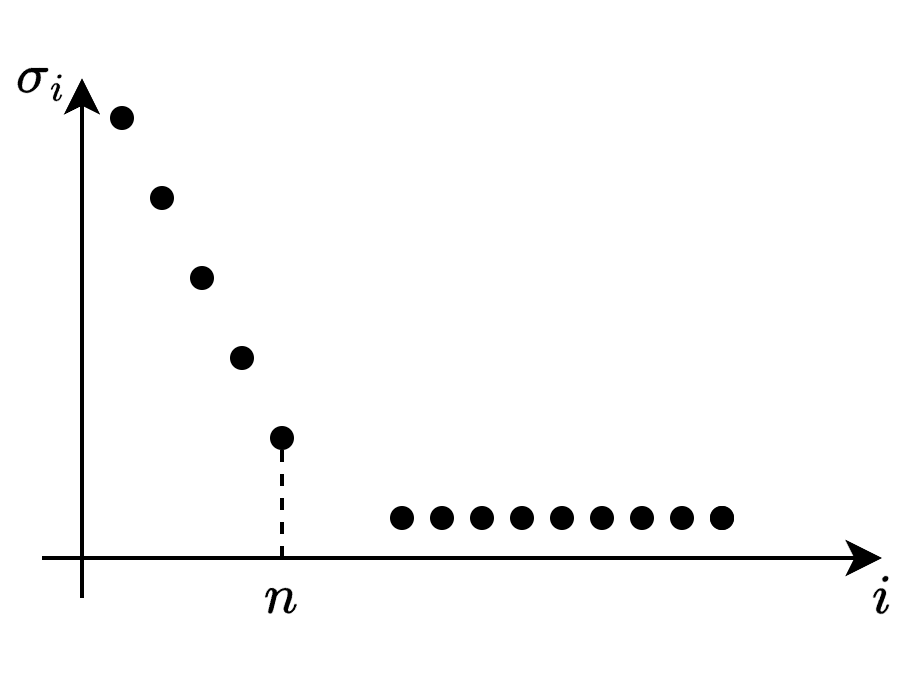
\includegraphics[width=0.4\linewidth]{images/qd1.png}
            \caption{Graphical representation of the ideal singular values}
        \end{figure}
        In the ideal scenario depicted above, there's a clear jump between the constant and decreasing parts of the graph, indicating the estimated order of the system $n$.
        However, in real-world scenarios, the graph might look more like this:
        \begin{figure}[H]
            \centering
            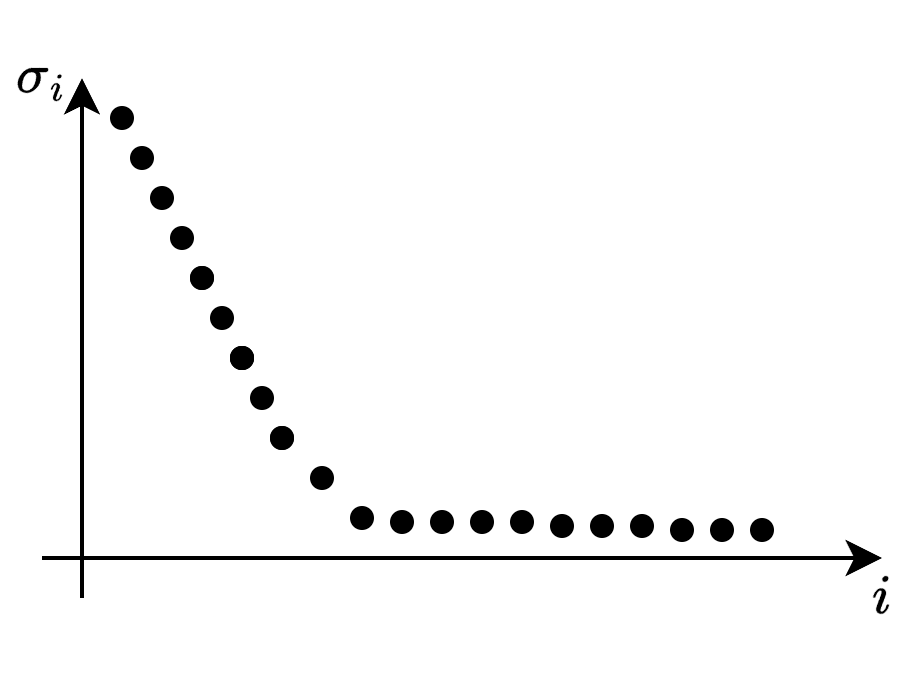
\includegraphics[width=0.4\linewidth]{images/qd2.png}
            \caption{Graphical representation of the real singular values}
        \end{figure}
        In such cases, we don't see a distinct jump but rather a knee in the graph. 
        The order of the system can lie at multiple points within this knee.
        Once we select an order, say $n$, we can cut the plot into two parts: the left containing the singular values of the system and the right containing the singular values of the noise.
        Typically, $n \ll q$. 

        We then proceed to cut the Hankel matrix at $n$ to obtain:
        \begin{figure}[H]
            \centering
            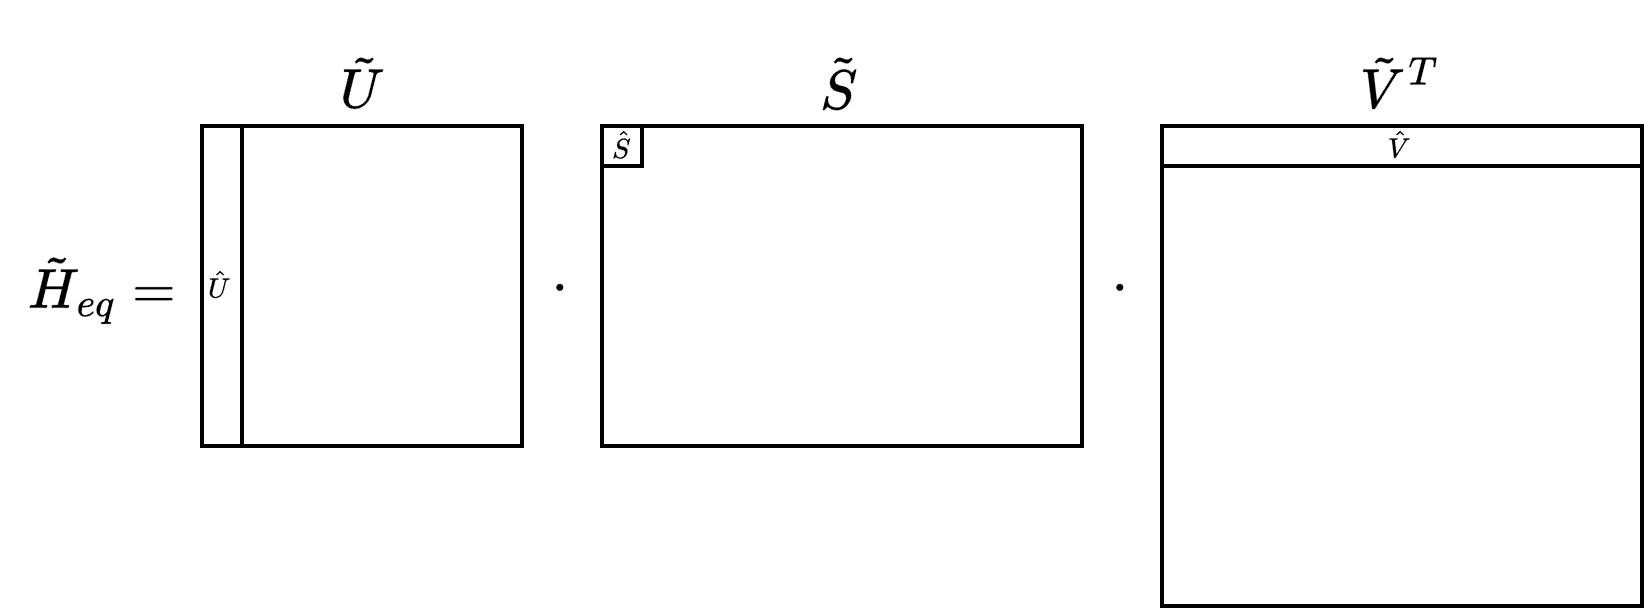
\includegraphics[width=0.75\linewidth]{images/hankel.png}
            \caption{Hankel matrix cutting}
        \end{figure}
        Now we define the reduced matrix:
        \[\hat{\mathbf{H}}_{qd}=\hat{\mathbf{U}}\hat{\mathbf{S}}\hat{\mathbf{V}}^T\]
        At this stage, we have:
        \[\tilde{\mathbf{H}}_{qd}=\hat{\mathbf{H}}_{qd}+{\mathbf{H}}_{\text{res}_{qd}}\]
        Where the rank of $\tilde{\mathbf{H}}_{qd}$ and ${\mathbf{H}}_{\text{res}_{qd}}$ is $q$, while the rank of $\hat{\mathbf{H}}_{qd}$ is $n$, indicating a significant rank reduction from $q$ to $n$. 
    \item Estimation of matrices $\hat{\mathbf{F}}$, $\hat{\mathbf{G}}$, and $\hat{\mathbf{H}}$  from the clean matrix $\tilde{\mathbf{H}}_{qd}$. 
        We start by decomposing $\hat{H}_{qd}$ as follows: 
        \[\hat{\mathbf{H}}_{qd}=\hat{\mathbf{U}}\hat{\mathbf{S}}\hat{\mathbf{V}}^T=\hat{\mathbf{U}}\sqrt{\hat{\mathbf{S}}}\sqrt{\hat{\mathbf{S}}}\hat{\mathbf{V}}^T\]
        We define:
        \[\hat{\mathbf{O}}=\hat{\mathbf{U}}\sqrt{\hat{\mathbf{S}}}\]
        \[\hat{\mathbf{R}}=\sqrt{\hat{\mathbf{S}}}\hat{\mathbf{V}}^T\]
        Therefore:
        \[\hat{\mathbf{H}}_{qd}=\hat{\mathbf{O}}\cdot\hat{\mathbf{R}}\]
        Where $\hat{\mathbf{O}}$ and $\hat{\mathbf{R}}$ are the extended observability and controllability matrices of the system, respectively.
        The first row of $\hat{\mathbf{O}}$ and the first column of $\hat{\mathbf{R}}$ represent $\hat{\mathbf{H}}$ and $\hat{\mathbf{G}}$, respectively.
        
        Next, we formulate two submatrices, $\mathbf{O}_1$ and $\mathbf{O}_2$, by excluding the last and first rows of $\hat{\mathbf{O}}$, respectively. 
        It's worth noting that $\mathbf{O}_1$ and $\mathbf{O}_2$ are square matrices due to the shift invariance property.
        
        Consequently, $\mathbf{O}_2=\mathbf{O}_1\cdot \hat{\mathbf{F}}$.
        Since $\mathbf{O}_1$ is rectangular and not directly invertible, $\hat{\mathbf{F}}$ can be determined as:
        \[\mathbf{O}_2=\mathbf{O}_1\cdot \hat{\mathbf{F}} \rightarrow \mathbf{O}_1^T\mathbf{O}_2=\mathbf{O}_1\mathbf{O}_1^T\cdot \hat{\mathbf{F}} \rightarrow \hat{\mathbf{F}}=\left(\mathbf{O}_1^T\mathbf{O}_1\right)^{-1}\mathbf{O}_1^T\mathbf{O}_2\]
\end{enumerate}
\begin{property}
    The optimality of the 4SID algorithm stems from the Singular Value Decomposition, which achieves an optimal reduction in rank.
\end{property}